\PassOptionsToPackage{unicode}{hyperref}
\documentclass[aspectratio=1610, professionalfonts, 9pt]{beamer}

\usefonttheme[onlymath]{serif}
\usetheme[showtotalframes]{tudo}

\ifluatex
\usepackage{polyglossia}
\setmainlanguage{german}
\else
\ifxetex
\usepackage{polyglossia}
\setmainlanguage{german}
\else
\usepackage[german]{babel}
\fi
\fi


% Mathematik
\usepackage{amsmath}
\usepackage{amssymb}
\usepackage{mathtools}
\usepackage{cancel}
\usepackage{siunitx}

\usepackage{hyperref}
\usepackage{bookmark}

% Bibliographie 
\usepackage[
  backend=biber,   
  autolang=hyphen,
  citestyle=verbose, 
  giveninits=true,
]{biblatex}
\addbibresource{references.bib} 
\DefineBibliographyStrings{german}{andothers = {{et\,al\adddot}}}

% Tabellen
\usepackage{booktabs}

%%%%%%%%%%%%%%%%%%%%%%%%%%%%%%%%%%%%%%%%%%%%%%%%%%%%%%%%%%%%%%%%%%%%%%%%%%%%%%%%
%%%%%-------------Hier Titel/Autor/Grafik/Lehrstuhl eintragen--------------%%%%%
%%%%%%%%%%%%%%%%%%%%%%%%%%%%%%%%%%%%%%%%%%%%%%%%%%%%%%%%%%%%%%%%%%%%%%%%%%%%%%%%

%Titel:
\title{Gamma/Hadron-Seperation bei FACT}
%Autor
\author[M.~Sackel]{Maximilian Sackel}
%Lehrstuhl/Fakultät
\institute[Experimental Physics 5]{Experimental Physiks 5b \\  Astroteilchenphysik}
%Titelgrafik 
\titlegraphic{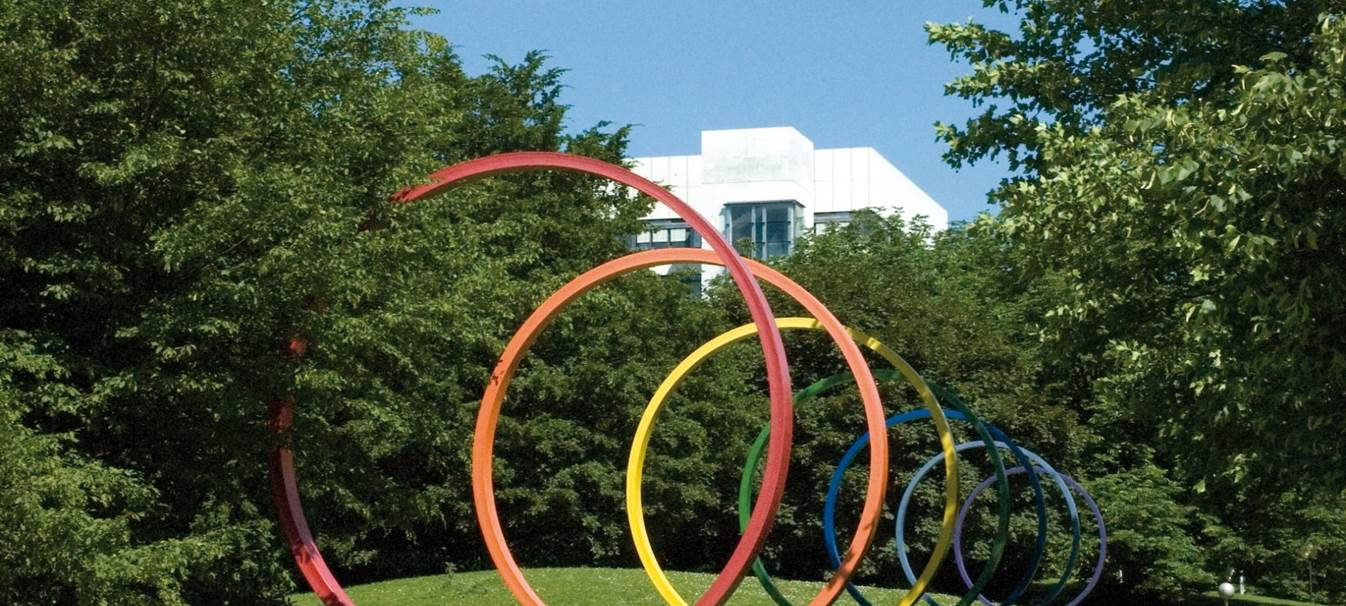
\includegraphics[width=0.7\textwidth]{images/tudo-title-2.jpg}}


\begin{document}

\maketitle

\section{Basics}
\begin{frame}
  \begin{figure}
	\centering
	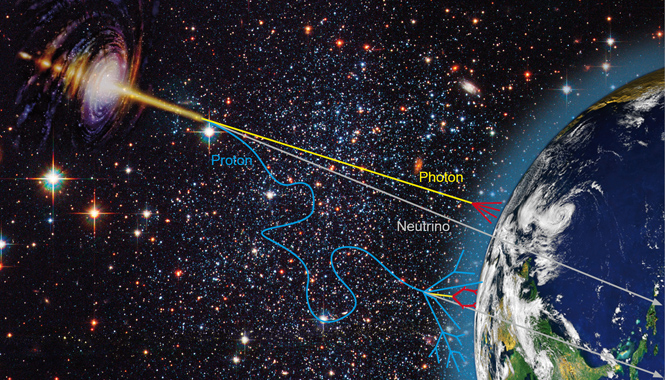
\includegraphics[width=0.8\textwidth]{./images/sources-detection.jpg} \\
	\caption{\cite{Overview}}
  \end{figure}
\end{frame}

\begin{frame}
  \begin{columns}
	\column{.3\textwidth}
	\begin{figure}
	  \centering
	  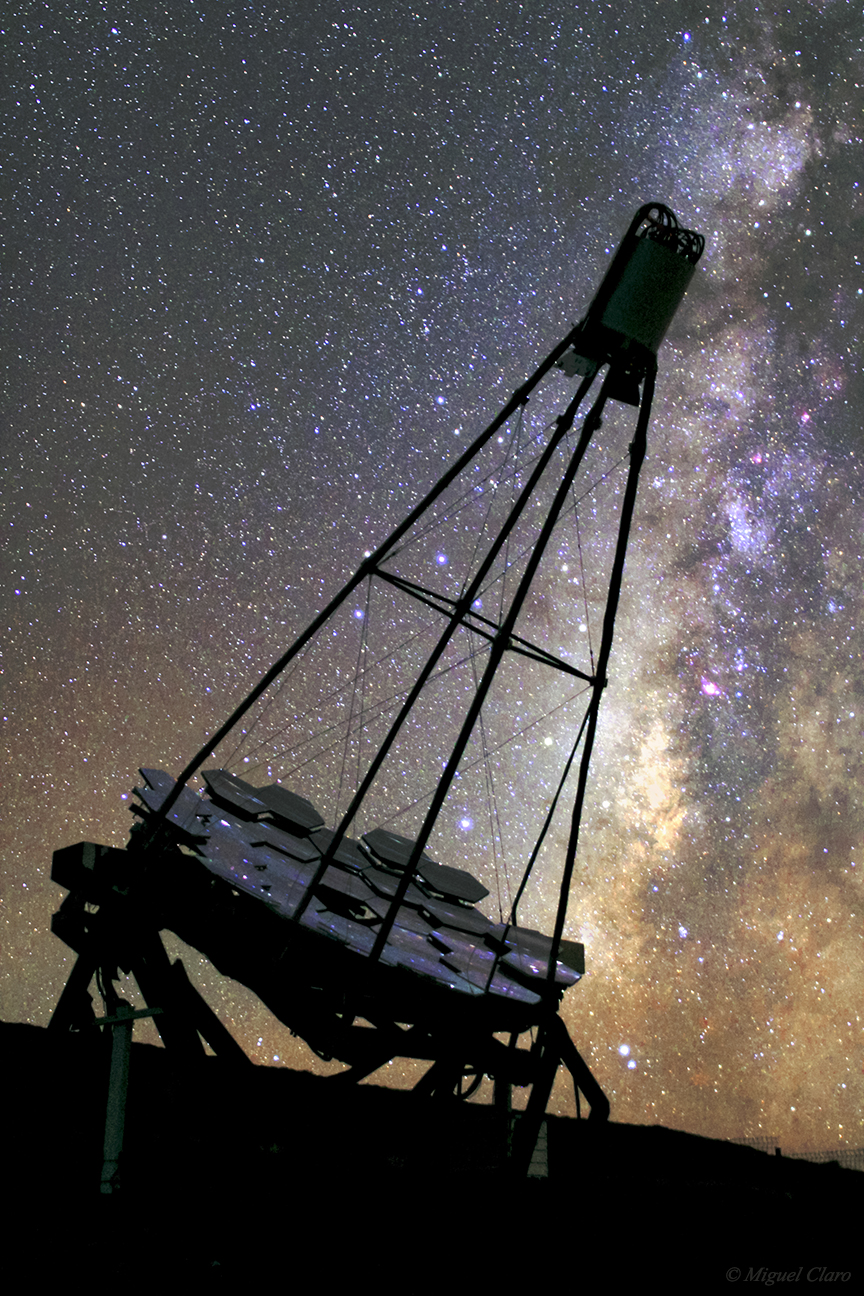
\includegraphics[height=0.8\textheight]{./images/FACT.jpg}
	  \caption{\cite{FACT}}
	\end{figure}
	\column{.7\textwidth}
	\only<1>{
	\Huge
	\centering
	\textbf{F}irst G-\textbf{A}PD \textbf{C}herenkov \textbf{T}elescope
  	}
	\only<2>{
	  \begin{figure}
		\centering
		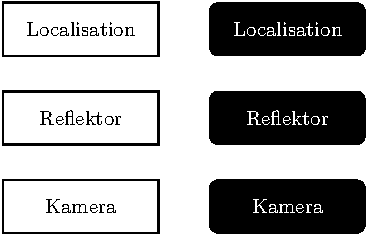
\includegraphics[height=0.8\textheight]{./tikz/FACT/FACT.pdf}
	  \end{figure}
	}
  \end{columns}
\end{frame}

\begin{frame}
  \begin{columns}
	\column{.2\textwidth}
	\begin{figure}
	  \centering
	  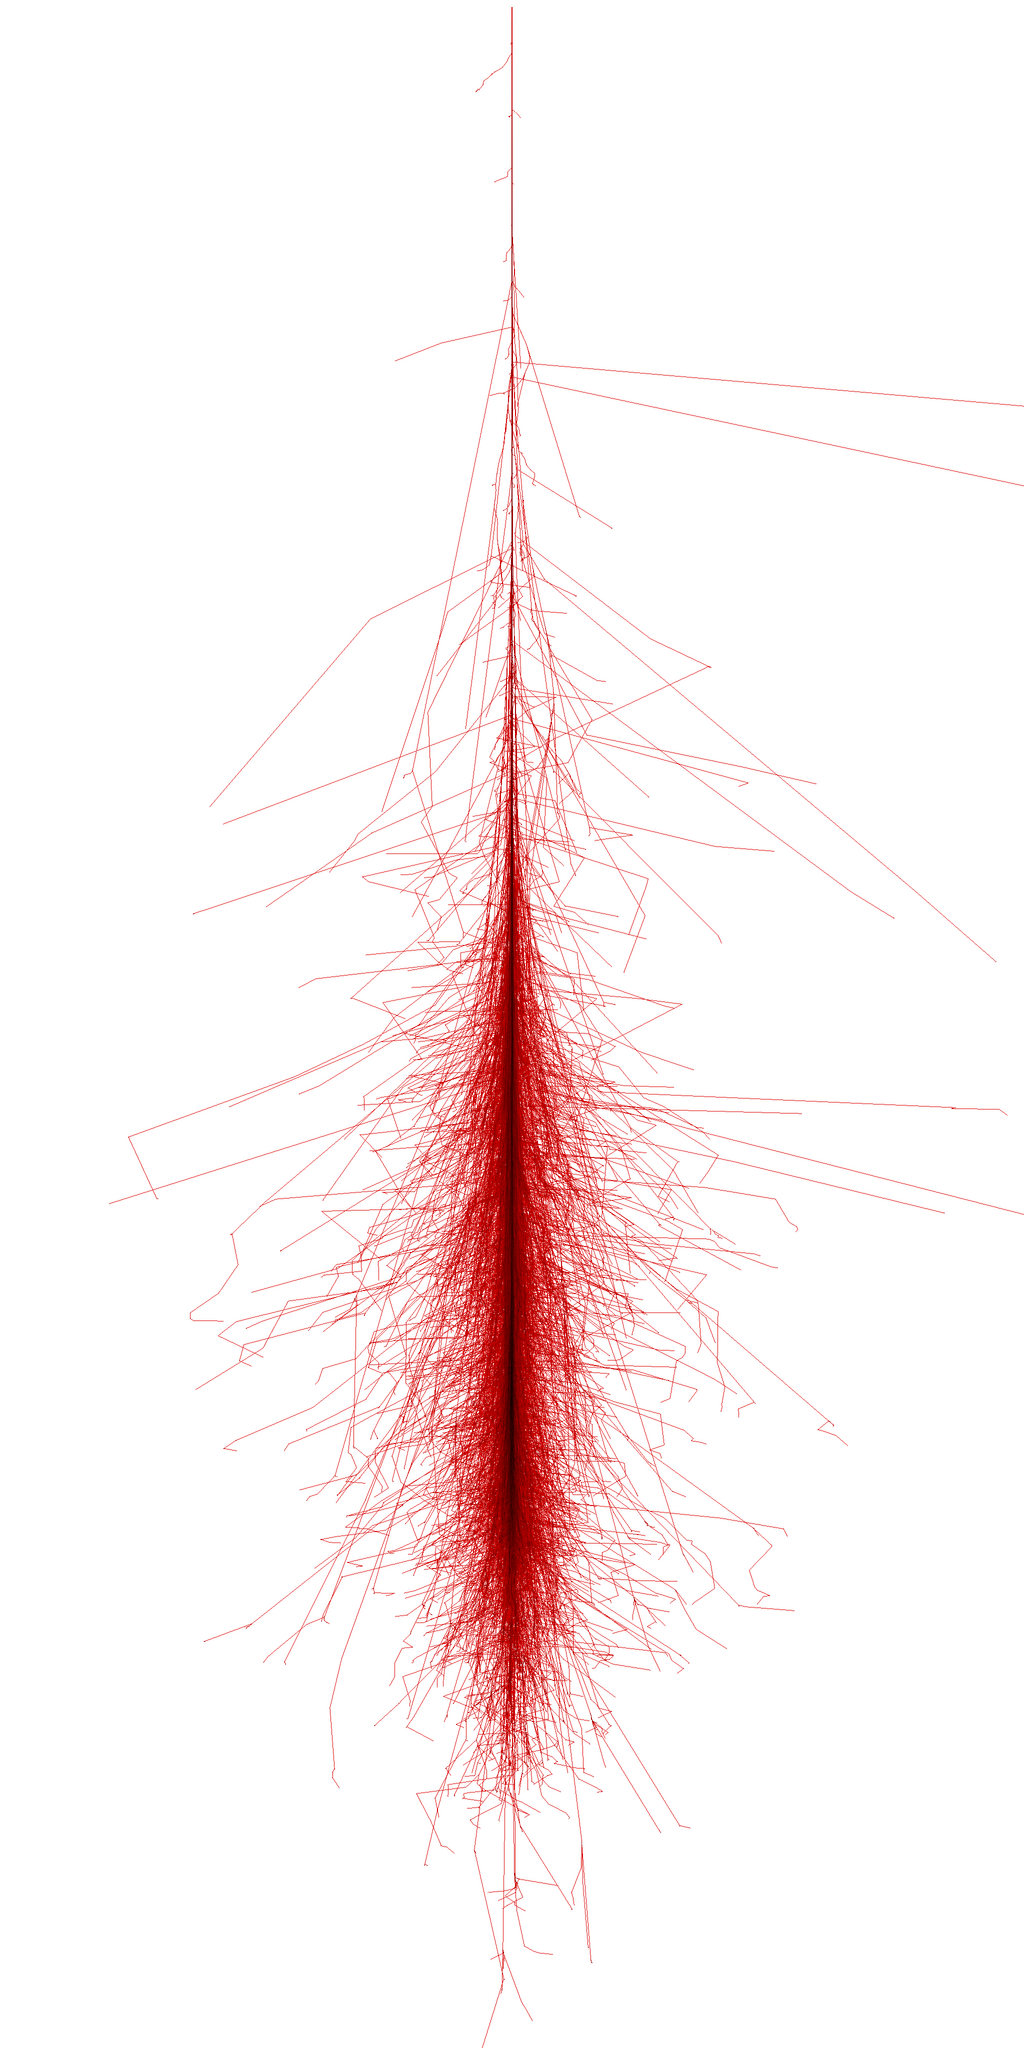
\includegraphics[width=\textwidth]{./images/photon_100GeV.png}
	  \caption{\cite{FACT}}
	\end{figure}
	\column{.3\textwidth}
	\begin{eqnarray*}
	  \gamma \rightarrow& e^{+} + e^{-} \\
	  e^{+} \rightarrow& e^{+'} + \gamma \\
	  e^{-} \rightarrow& e^{-'} + \gamma 
	\end{eqnarray*}
	\column{.2\textwidth}
	\begin{figure}
	  \centering
	  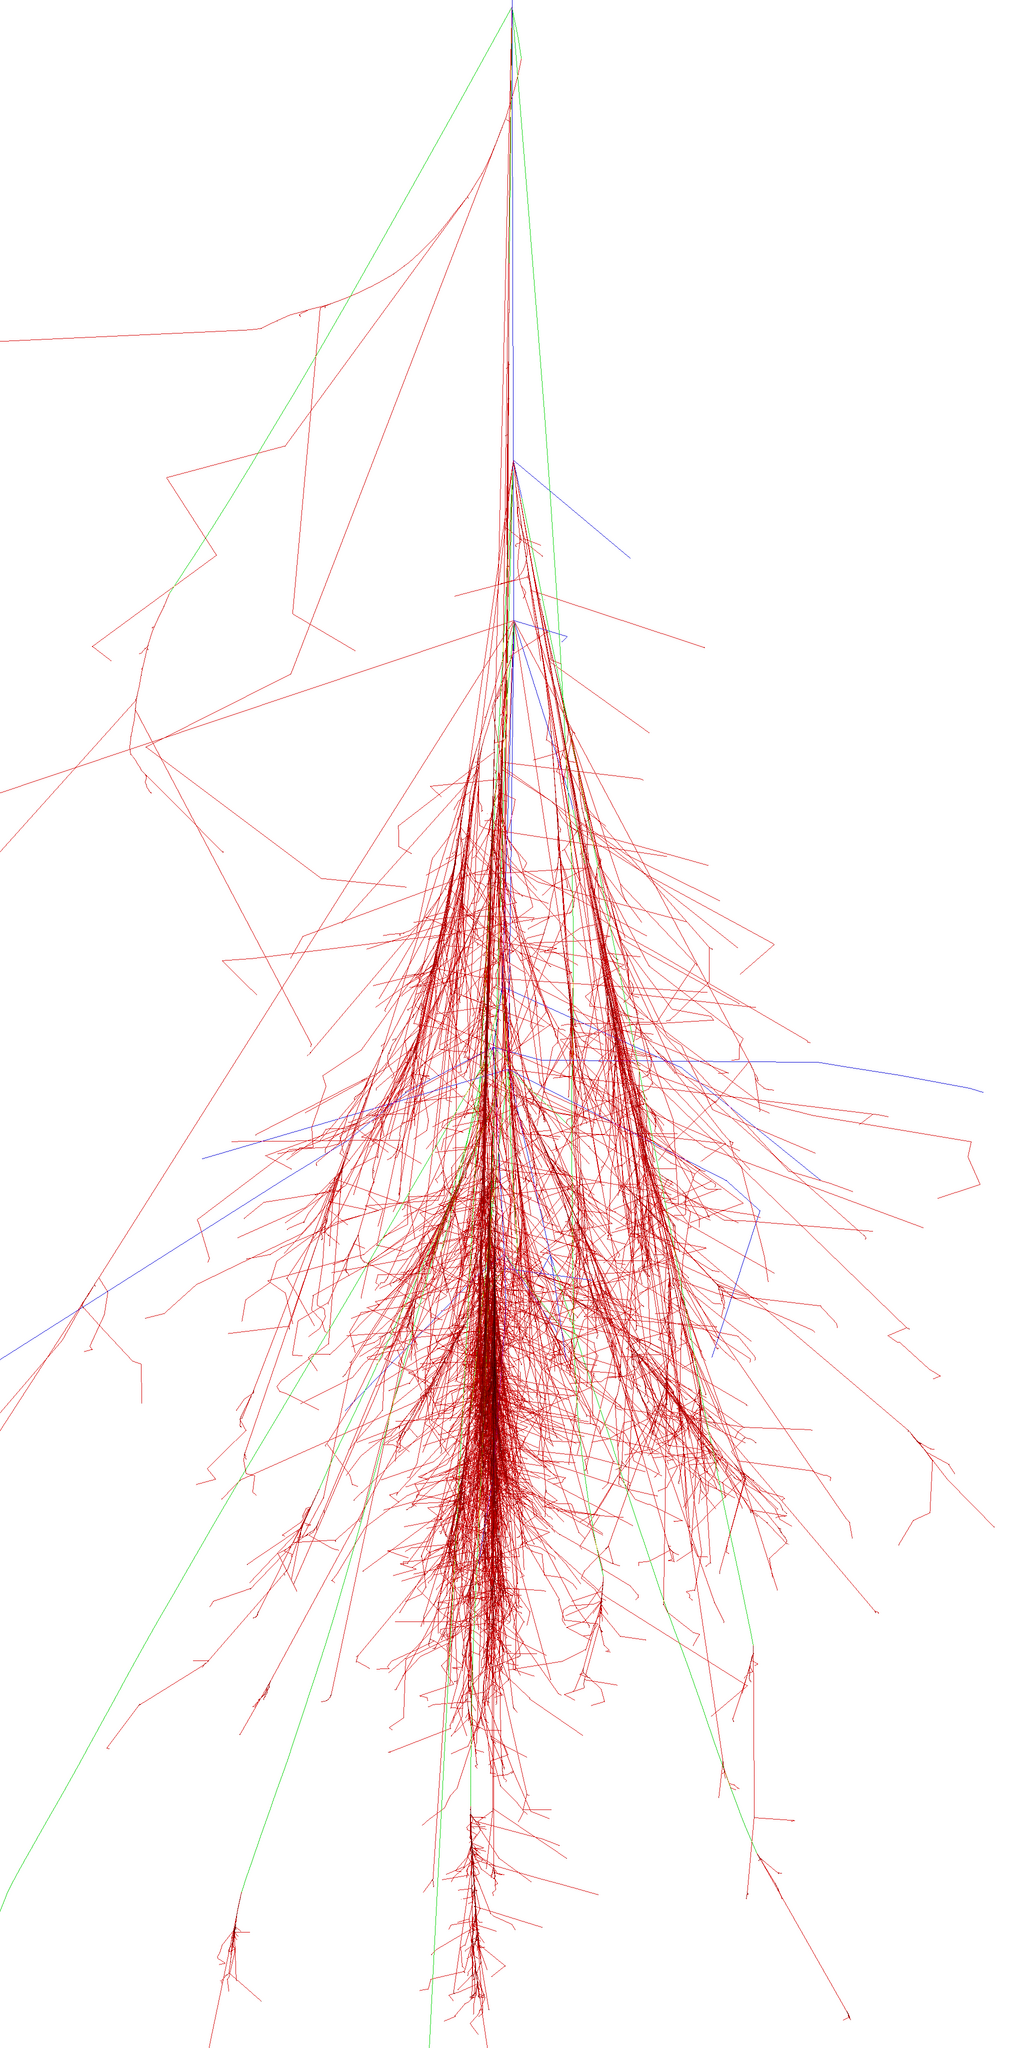
\includegraphics[width=\textwidth]{./images/proton_100GeV.png}
	  \caption{\cite{FACT}}
	\end{figure}
	\column{.3\textwidth}
	\begin{eqnarray*}
	  \pi^{0} \rightarrow& \gamma + \gamma \\
	  \pi^{+} \rightarrow& \mu^{+} + \nu_{\mu} \\
	  \pi^{-} \rightarrow& \mu^{-} + \bar{\nu}_{\mu}
	\end{eqnarray*}
  \end{columns}
\end{frame}

\begin{frame}
  \begin{columns}
	\column{.5\textwidth}
	\begin{figure}
	  \centering
	  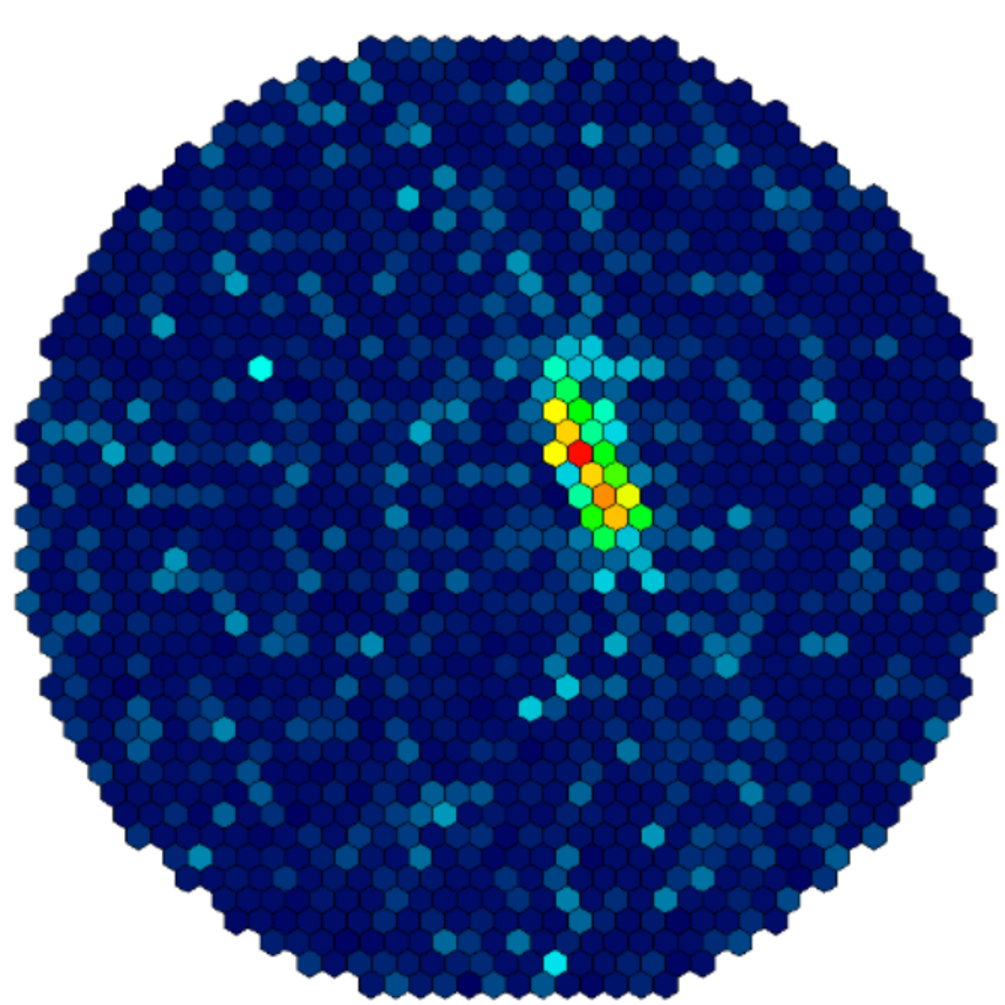
\includegraphics[height=0.8\textheight]{./images/Gamma.pdf}
	  \caption{\cite{FACT}}
	\end{figure}
	\column{.5\textwidth}
	\begin{figure}
	  \centering
	  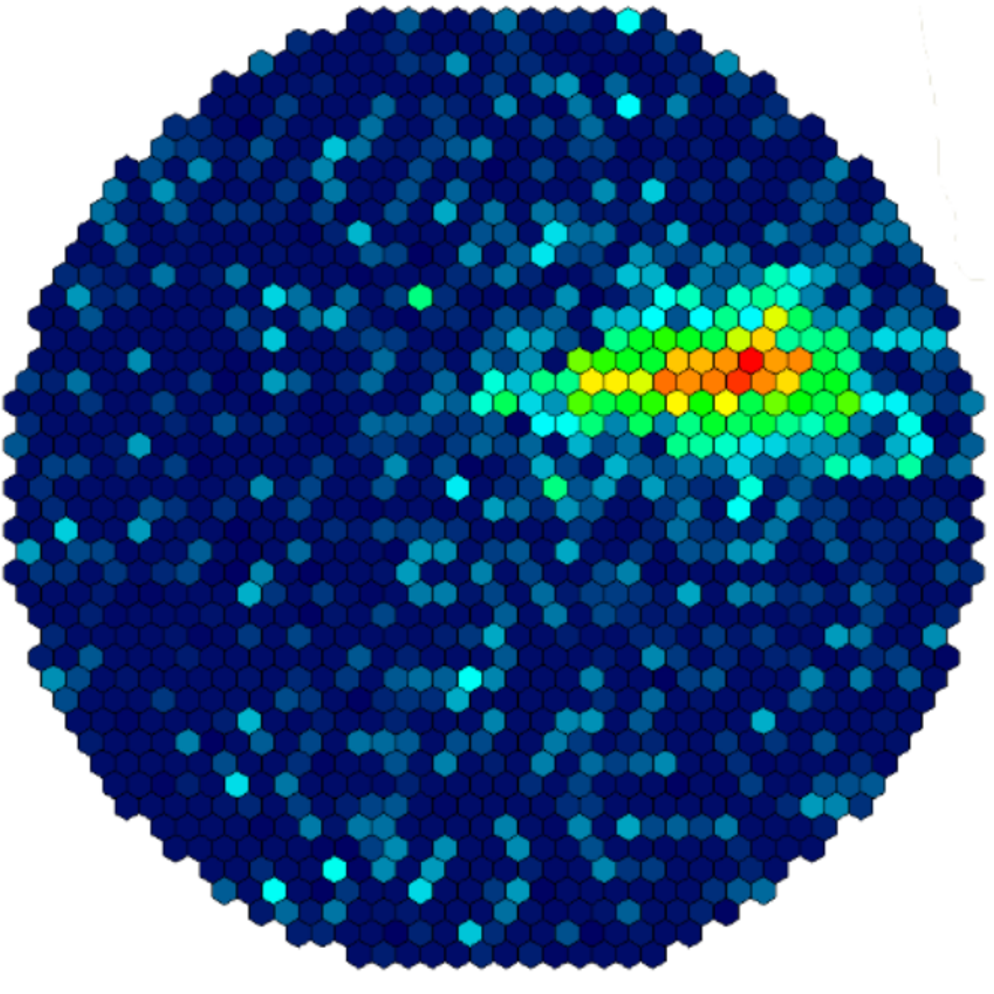
\includegraphics[height=0.8\textheight]{./images/Hadron.pdf}
	  \caption{\cite{FACT}}
	\end{figure}
  \end{columns}
\end{frame}


\begin{frame}
  \begin{columns}
	\column{.5\textwidth}
	\begin{figure}
	  \centering
	  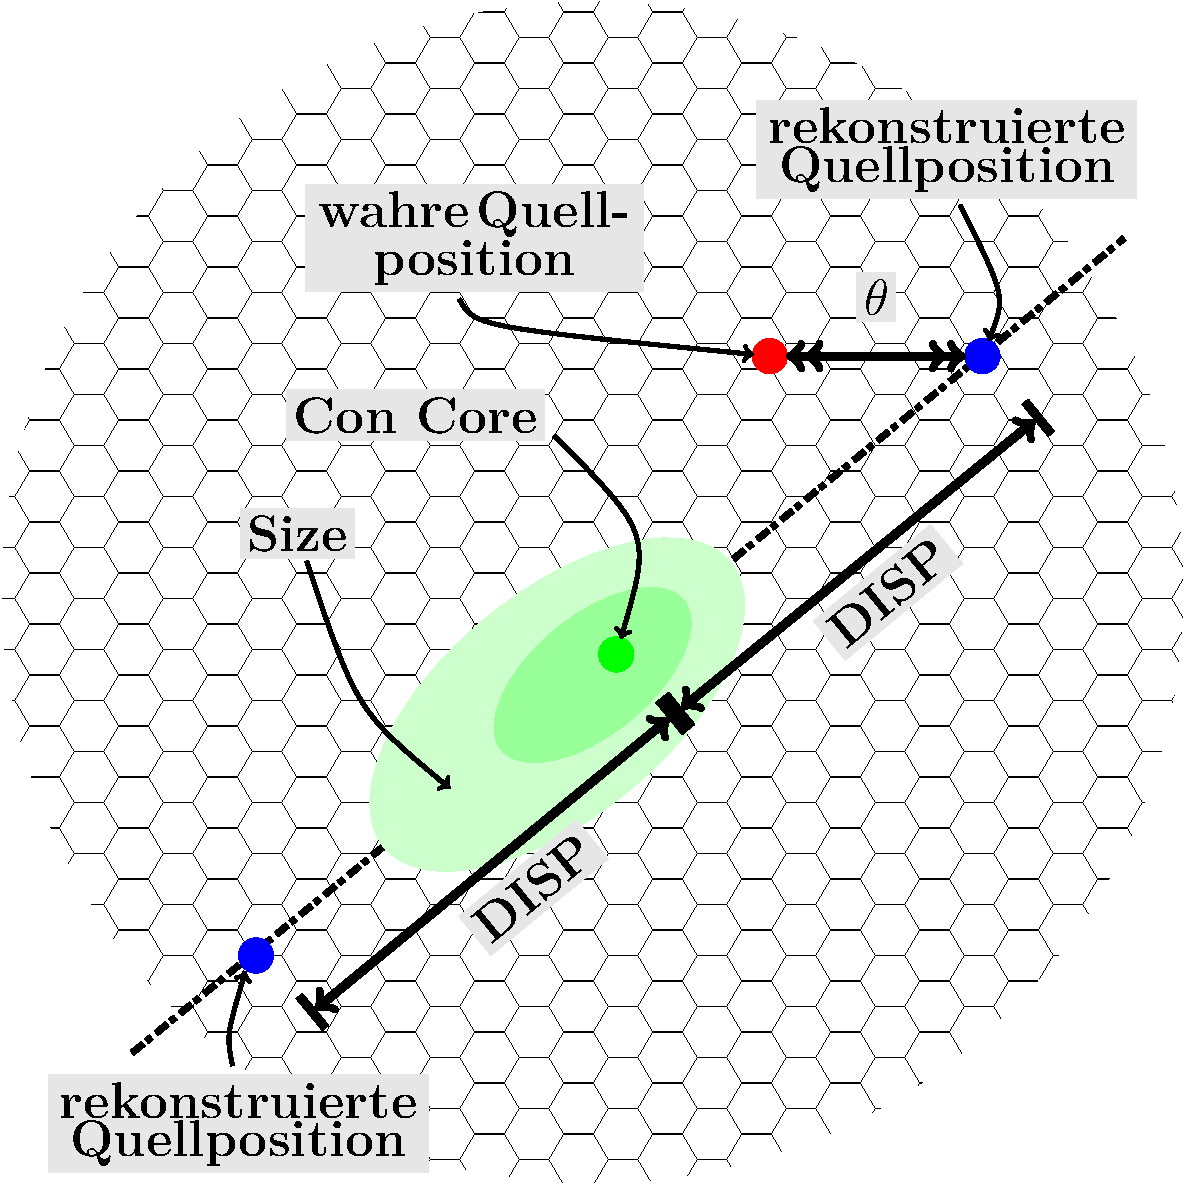
\includegraphics[height=0.8\textheight]{./images/camera.pdf}
	\end{figure}
	\column{.5\textwidth}
	\begin{itemize}
		\item berechne Feature (Hillas Parameter) des Kamerabildes
		\item Feature werden zum Klassifizieren benoetigt
		\item Vorzeichen des Schauers nicht eindeutig
	\end{itemize}
  \end{columns}
\end{frame}

\begin{frame}
  \begin{columns}
	\column{.5\textwidth}
	\begin{figure}
	  \centering
	  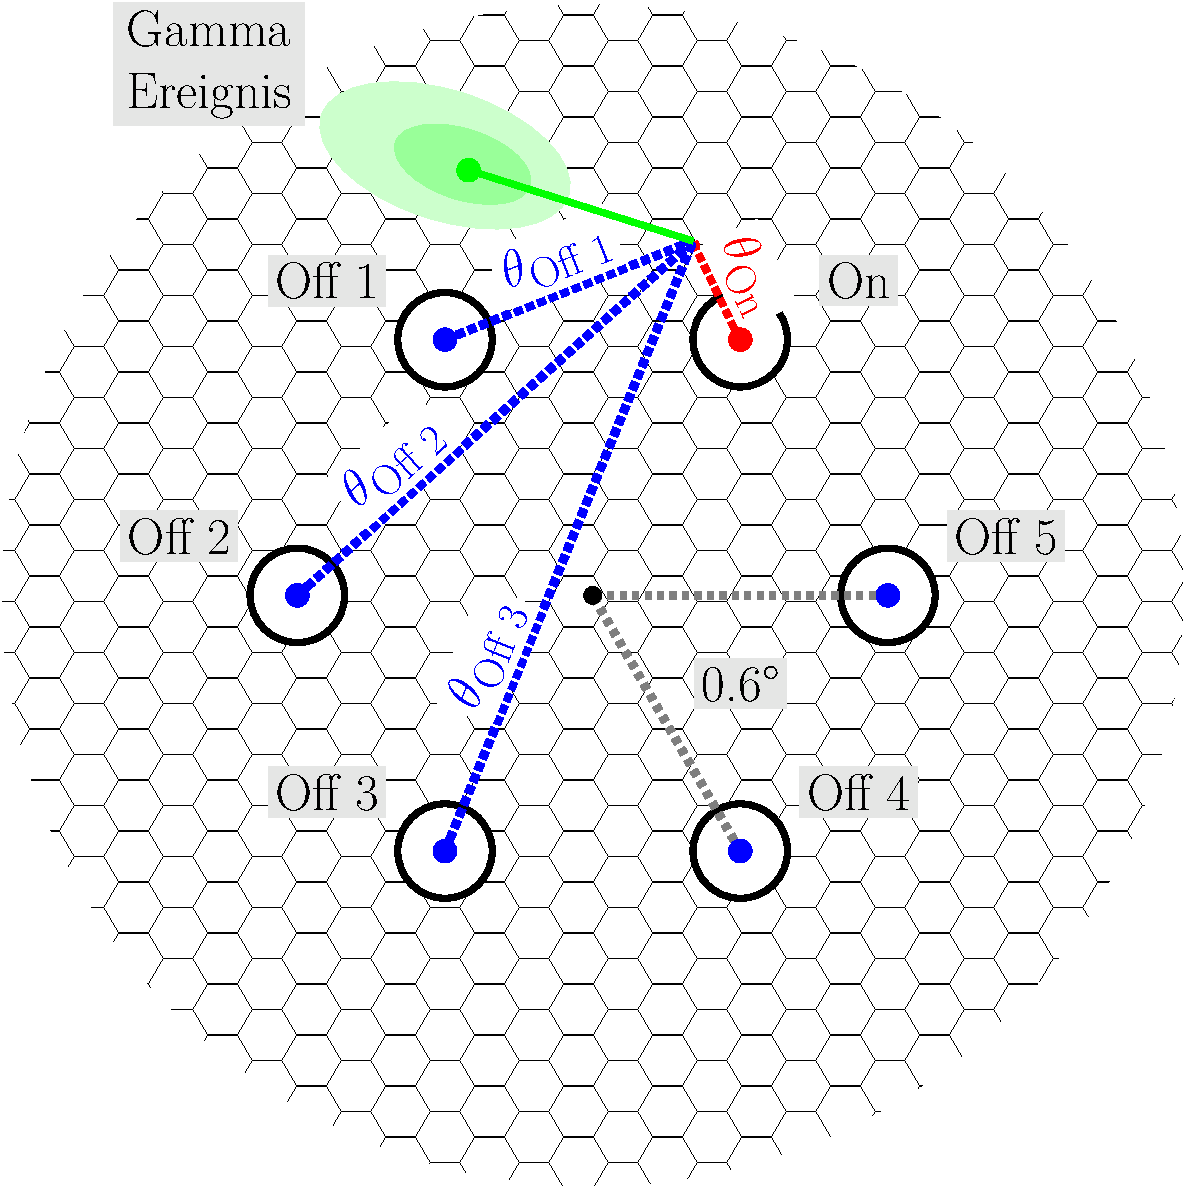
\includegraphics[height=0.8\textheight]{./images/wobble.pdf}
	\end{figure}
	\column{.5\textwidth}
	\begin{itemize}
		\item FACT nimmt keine OFF-Daten
		\item Daten werden im Wobble Modus genommen
	\end{itemize}
  \end{columns}
\end{frame}

\begin{frame}
  \begin{block}{Seperation}<1-2>
	\begin{figure}
	  \centering
	  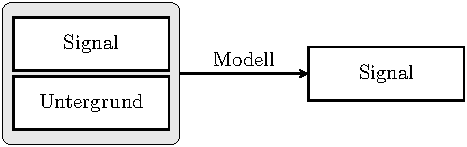
\includegraphics[scale=1]{./tikz/Target/Target.pdf}
	\end{figure}
  \end{block}
  \begin{block}{Simulierte Daten}<2>
	\begin{figure}
	  \centering
	  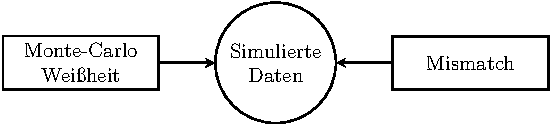
\includegraphics[scale=1]{./tikz/Mismatch/Mismatch.pdf}
	\end{figure}
  \end{block}
\end{frame}

\section{Modelle}
\begin{frame}{Entscheidungsbaum}
  \begin{columns}
	\column{.4\textwidth}
	\begin{figure}
	  \centering
	  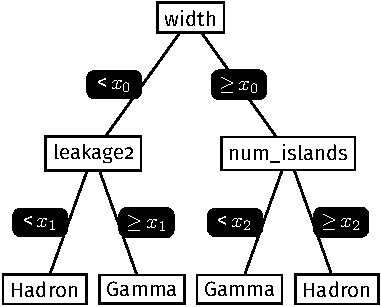
\includegraphics[width=\textwidth]{./tikz/Tree/Tree.pdf}
	\end{figure}
	\column{.6\textwidth}
	\begin{itemize}
	  \item Verknüpfte Abfragen 
	  \item Loss-function
	  \item Beschränkung der Komplexität 
	\end{itemize}
	\begin{table}	  
	  \centering
	  \begin{tabular}{c c c c c c}
		\toprule
		Ereignis & width & leakage2 & num\_islands & \dots & Konfi. \\ 
		\cmidrule(r){1-1} 	\cmidrule{2-5} \cmidrule(l){6-6}
		1 & \num{4.2}  & \num{0.4}  & \num{3} & \dots & \num{0.12} \\
		2 & \num{3.8}  & \num{0.0}  & \num{2} & \dots & \num{0.56} \\
		3 & \num{15.3} & \num{0.8} 	& \num{1} & \dots & \num{0.08} \\
		4 & \num{7.7}  & \num{0.1}  & \num{1} & \dots & \num{0.43} \\
		5 & \num{6.2}  & \num{0.0}  & \num{1} & \dots & \num{0.85} \\
		\bottomrule
	  \end{tabular}
	\end{table}
  \end{columns}
\end{frame}

\begin{frame}{Random Forest}
  \begin{columns}
	\column{.5\textwidth}
	\begin{figure}
	  \centering
	  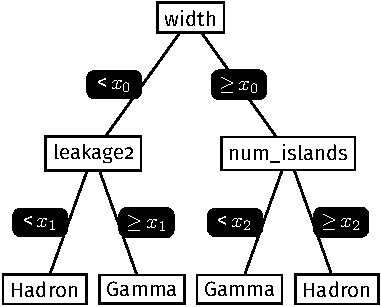
\includegraphics[scale=1]{./tikz/Tree/Tree.pdf}
	\end{figure}
	\column{.5\textwidth}
	\begin{figure}
	  \centering
	  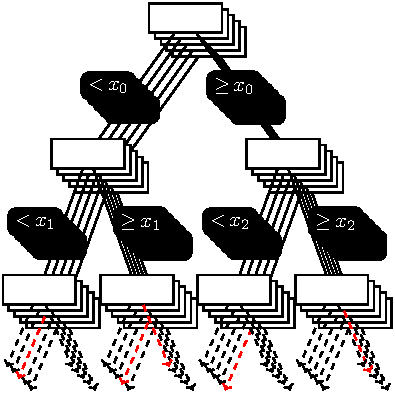
\includegraphics[scale=1]{./tikz/RandomForest/RandomForest.pdf}
	\end{figure}
  \end{columns}
\end{frame}

\begin{frame}{Random Forest}
  \begin{columns}
	\column{.4\textwidth}
	\begin{table}
	  \centering
	  \begin{tabular}{c c}
		\toprule
		Ereignis & Konfi. \\
		\cmidrule(r){1-1} \cmidrule(l){2-2}
		1 & \num{0.12} \\
		2 & \num{0.56} \\
		3 & \num{0.08} \\
		4 & \num{0.43} \\
		5 & \num{0.85} \\
		\bottomrule
	  \end{tabular}
	\end{table}
	\column{.6\textwidth}
	\begin{table}
	  \centering
	  \begin{tabular}{c c c c c c}
		\toprule
		Ereignis & Konf$_{1}$ & Konf$_{2}$ & Konf$_{3}$ & \dots & $\Sigma_\text{i}$ Konf$_\text{i}$ \\
		\cmidrule(r){1-1} \cmidrule(lr){2-5} \cmidrule(l){6-6}
		1 & \num{0.12} & \num{0.01} & \num{0.08} & \dots & \num{0.06} \\
		2 & \num{0.40} & \num{0.66} & \num{0.53} & \dots & \num{0.56} \\
		3 & \num{0.02} & \num{0.17} & \num{0.10} & \dots & \num{0.08} \\
		4 & \num{0.41} & \num{0.42} & \num{0.42} & \dots & \num{0.43} \\
		5 & \num{0.96} & \num{0.81} & \num{0.85} & \dots & \num{0.85} \\
		\bottomrule
	  \end{tabular}
	\end{table}
  \end{columns}
\end{frame}

\begin{frame}{Boosted Trees}
  \begin{columns}
	\only<1>{\column{.4\textwidth}
	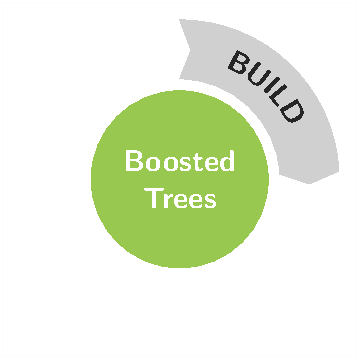
\includegraphics[width=\textwidth]{./tikz/BoostedTree/BoostedTree1.pdf}}
	\only<2>{\column{.4\textwidth}
	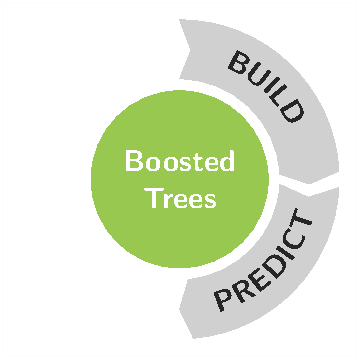
\includegraphics[width=\textwidth]{./tikz/BoostedTree/BoostedTree2.pdf}}
	\only<3>{\column{.4\textwidth}
	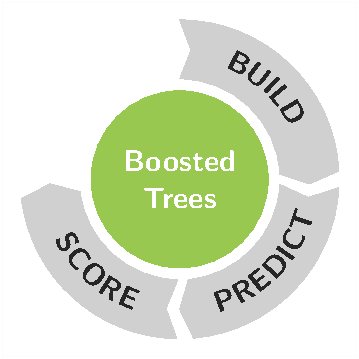
\includegraphics[width=\textwidth]{./tikz/BoostedTree/BoostedTree3.pdf}}
	\only<4>{\column{.4\textwidth}
	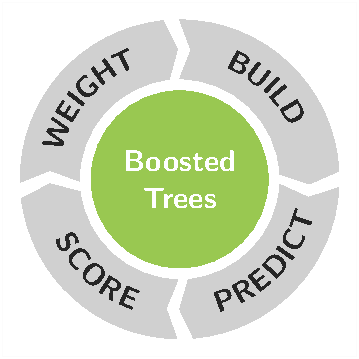
\includegraphics[width=\textwidth]{./tikz/BoostedTree/BoostedTree.pdf}}
	\column{.6\textwidth}
	\begin{itemize}
	  \item additives Training
	  \item höhere Gewichtung von Fehlklassifizierungen
	  \item ausgeglicherene Vorhersage
	  \item lässt sich nicht Parallelisieren
	  \item Modelle mit geringere Komplexität
	\end{itemize}
  \end{columns}
\end{frame}

\section{Blindtext}
\begin{frame}
  \frametitle{Hier steht eine lange, zweizeilige Headline
  \newline gefolgt von einem Blindtext}
  Dieser Text dient nur zur Veranschaulichung des Textsatzes. Niemand sollte jemals, aus keinem noch so gutem Grund, so viel Text auf eine Folie packen.

  Dies ist ein Blindtext. Dieser Text ist nicht dafür vorgesehen, den Betrachter in die Welt der Dunkelheit zu führen, sondern dafür, einfach etwas Leeres mit etwas Inhaltlosem zu füllen.

  Dies ist ein Blindtext. Dieser Text ist nicht dafür vorgesehen, den Betrachter in die Welt der Dunkelheit zu führen, sondern dafür, einfach etwas Leeres mit etwas Inhaltlosem zu füllen.

  Dies ist ein Blindtext. Dieser Text ist nicht dafür vorgesehen, den Betrachter in die Welt der Dunkelheit zu führen, sondern dafür, einfach etwas Leeres mit etwas Inhaltlosem zu füllen.
\end{frame}

\begin{frame}{title}
  \begin{enumerate}
	\item test
	\item test
  \end{enumerate}
\end{frame}

\begin{frame}{title}
  \begin{block}{title}
	ANlsnldas dkmadföonslkadm x
  \end{block}
 \end{frame}
\end{document}
